\documentclass[aspectratio=169]{beamer}

\usetheme{Madrid}
\usecolortheme{default}

\usepackage[T1]{fontenc}
\usepackage[utf8]{inputenc}
\usepackage{lmodern}
\usepackage{amsmath,amssymb}
\usepackage{graphicx}
\usepackage{booktabs}
\usepackage{tabularx}

\graphicspath{{figures/}{./}}

\title[AI-Ready HAPS--UAV Channel Model]{An AI-Ready Air-to-Ground Channel Model for HAPS--UAV Access Networks}
\author{Harsha Matadhikari}
\institute{Online PG Diploma in Advanced Communication Engineering with Quantum AI Integration \\ Indian Institute of Technology Delhi}
\date{}

\begin{document}

% ---------------------------------------------------------------
\begin{frame}
\titlepage
\end{frame}

% ---------------------------------------------------------------
\begin{frame}{Motivation}
\begin{itemize}
  \item A 3-HAPS equilateral-triangle constellation serves a ground footprint via
        \textbf{service} (2\,GHz), \textbf{backhaul} (38\,GHz), and two-hop
        \textbf{UAV relay} links.
  \item Distance-only link budgeting misses a key effect: co-channel
        interference from the other two HAPS makes SINR depend strongly on
        \emph{angular position}, not just distance.
  \item Static link-quality analysis cannot react to this, or to
        time-varying rain fades on the 38\,GHz backhaul.
  \item \textbf{AI Ready Model:} a validated channel model, an LSTM rain
        forecaster, and a DQN agent that learns real-time user--platform
        association -- evaluated honestly, including where it \emph{doesn't} win.
\end{itemize}

\vspace{4mm}
\begin{center}
\footnotesize
\textbf{Research flow:}\\[1mm]
\fbox{\parbox{0.27\textwidth}{\centering Attenuation \& channel models\\(FSPL, rain, fog, gas, scintillation, interference)}}
$\;\rightarrow\;$
\fbox{\parbox{0.22\textwidth}{\centering Baseline policies\\(random, max-SINR, max-throughput)}}
$\;\rightarrow\;$
\fbox{\parbox{0.27\textwidth}{\centering AI model\\(LSTM forecast + DQN) for\\platform selection \& positioning}}
\end{center}
\end{frame}

% ---------------------------------------------------------------
\begin{frame}{System Topology and Channel Model}
\begin{columns}[T]
\begin{column}{0.5\textwidth}
\vspace{-11mm}
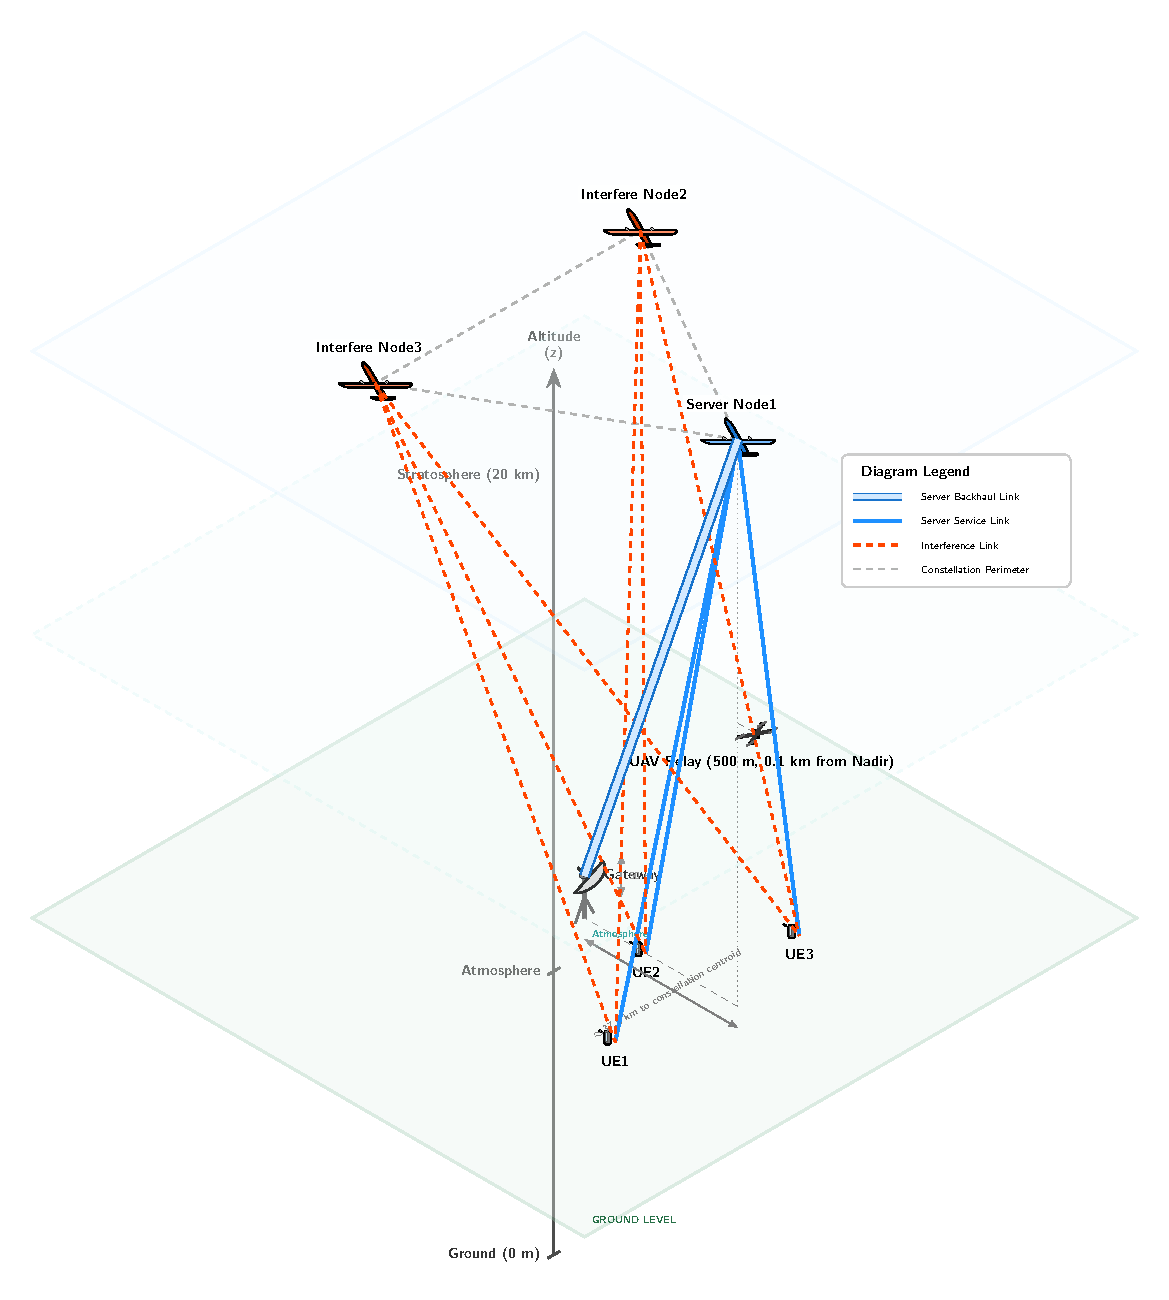
\includegraphics[width=\linewidth]{network_diagram_gw.pdf}
\end{column}
\begin{column}{0.5\textwidth}
\footnotesize
\textbf{Three link types:}
\begin{itemize}
  \item HAPS $\rightarrow$ UE (service, 2\,GHz)
  \item HAPS $\rightarrow$ Gateway (backhaul, 38\,GHz)
  \item HAPS $\rightarrow$ UAV $\rightarrow$ UE (relay; feeder hop at
        38\,GHz, UAV$\rightarrow$UE access hop at 2\,GHz)
\end{itemize}
\vspace{4mm}
\textbf{Channel model:}
\begin{itemize}
  \item Free-space path loss (HAPS tier)
  \item Building-blockage LoS/NLoS probability (UAV tier, Holis \& Pechac 2008)
  \item ITU-R rain, fog, gas, and scintillation losses (backhaul/feeder)
\end{itemize}
\vspace{2mm}
\scriptsize\textbf{Single relay UAV, fixed 0.1\,km from the serving HAPS's own nadir} (the Gateway occupies the centroid instead) --
not hovering beside whichever user it serves (next slide).
\end{column}
\end{columns}
\end{frame}

% ---------------------------------------------------------------
\begin{frame}{Path Loss and SINR vs.\ Distance}
\begin{columns}[T]
\begin{column}{0.34\textwidth}
\centering
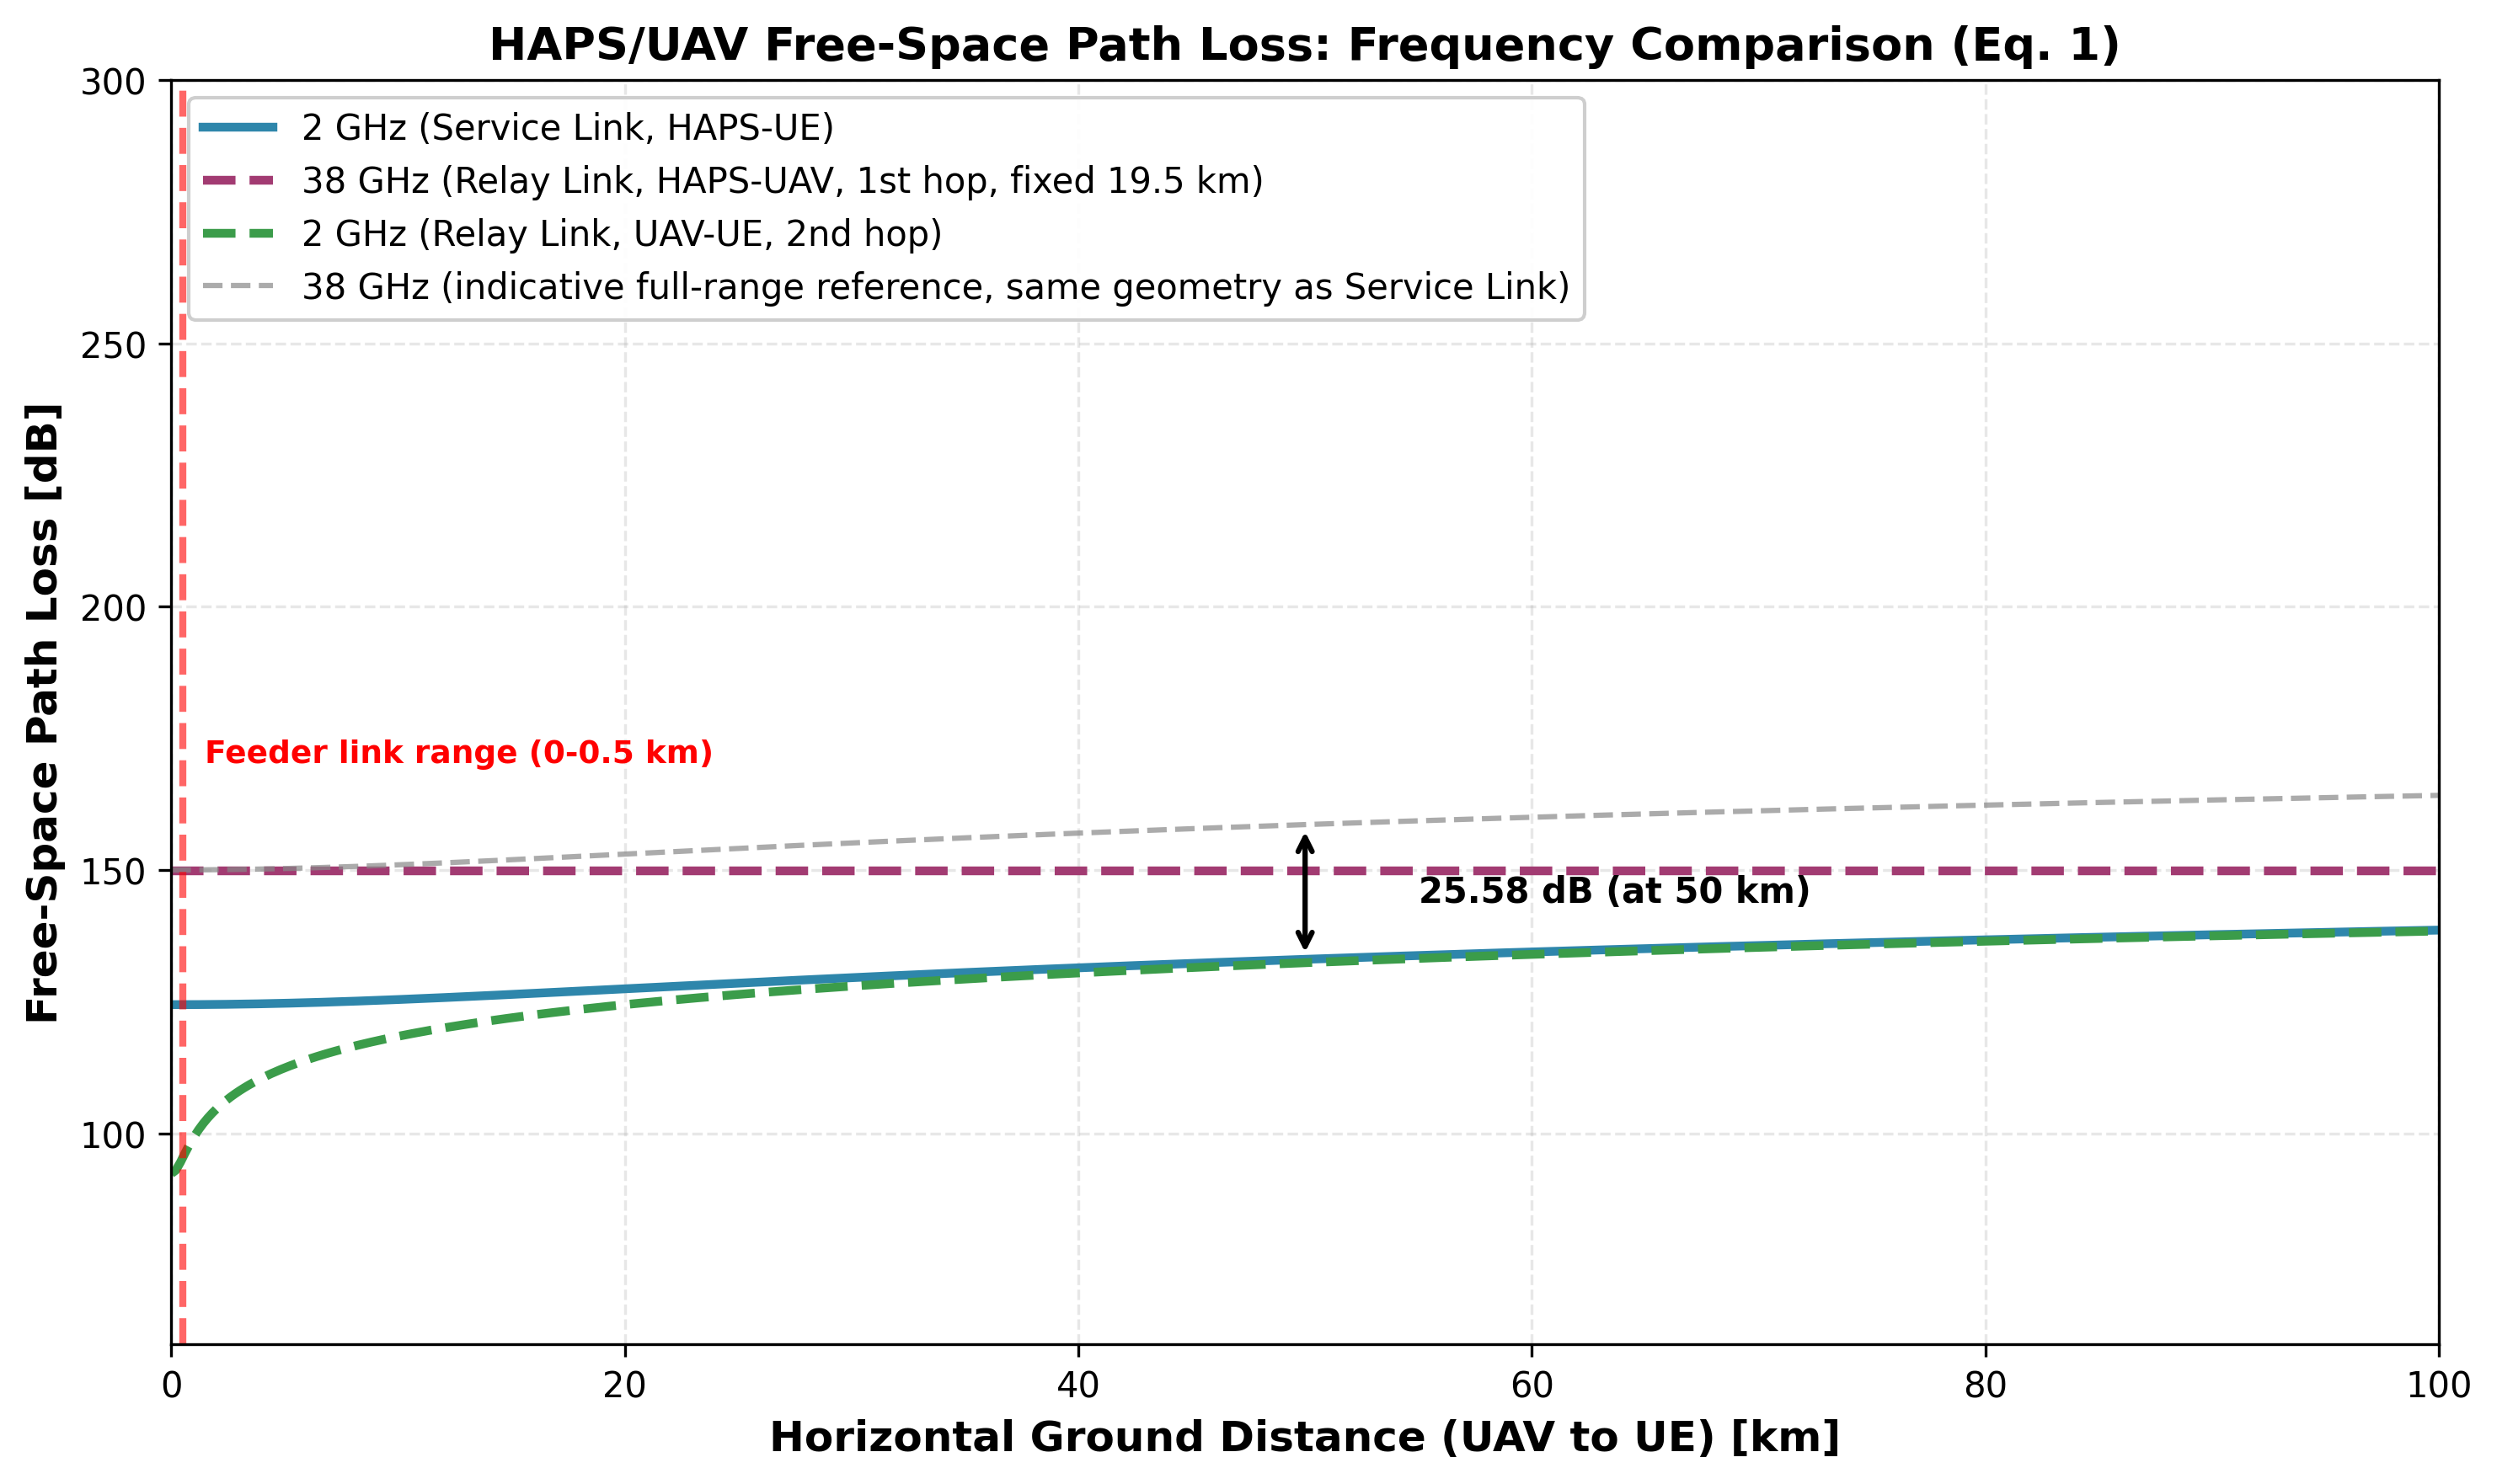
\includegraphics[width=\linewidth]{1b_haps_fspl_2ghz_vs_38ghz.png}\\
\scriptsize\textbf{FSPL vs.\ distance} -- same form for 2\,GHz and
38\,GHz; the feeder sits $\approx$25.6\,dB higher purely from the
frequency term.
\end{column}
\begin{column}{0.33\textwidth}
\centering
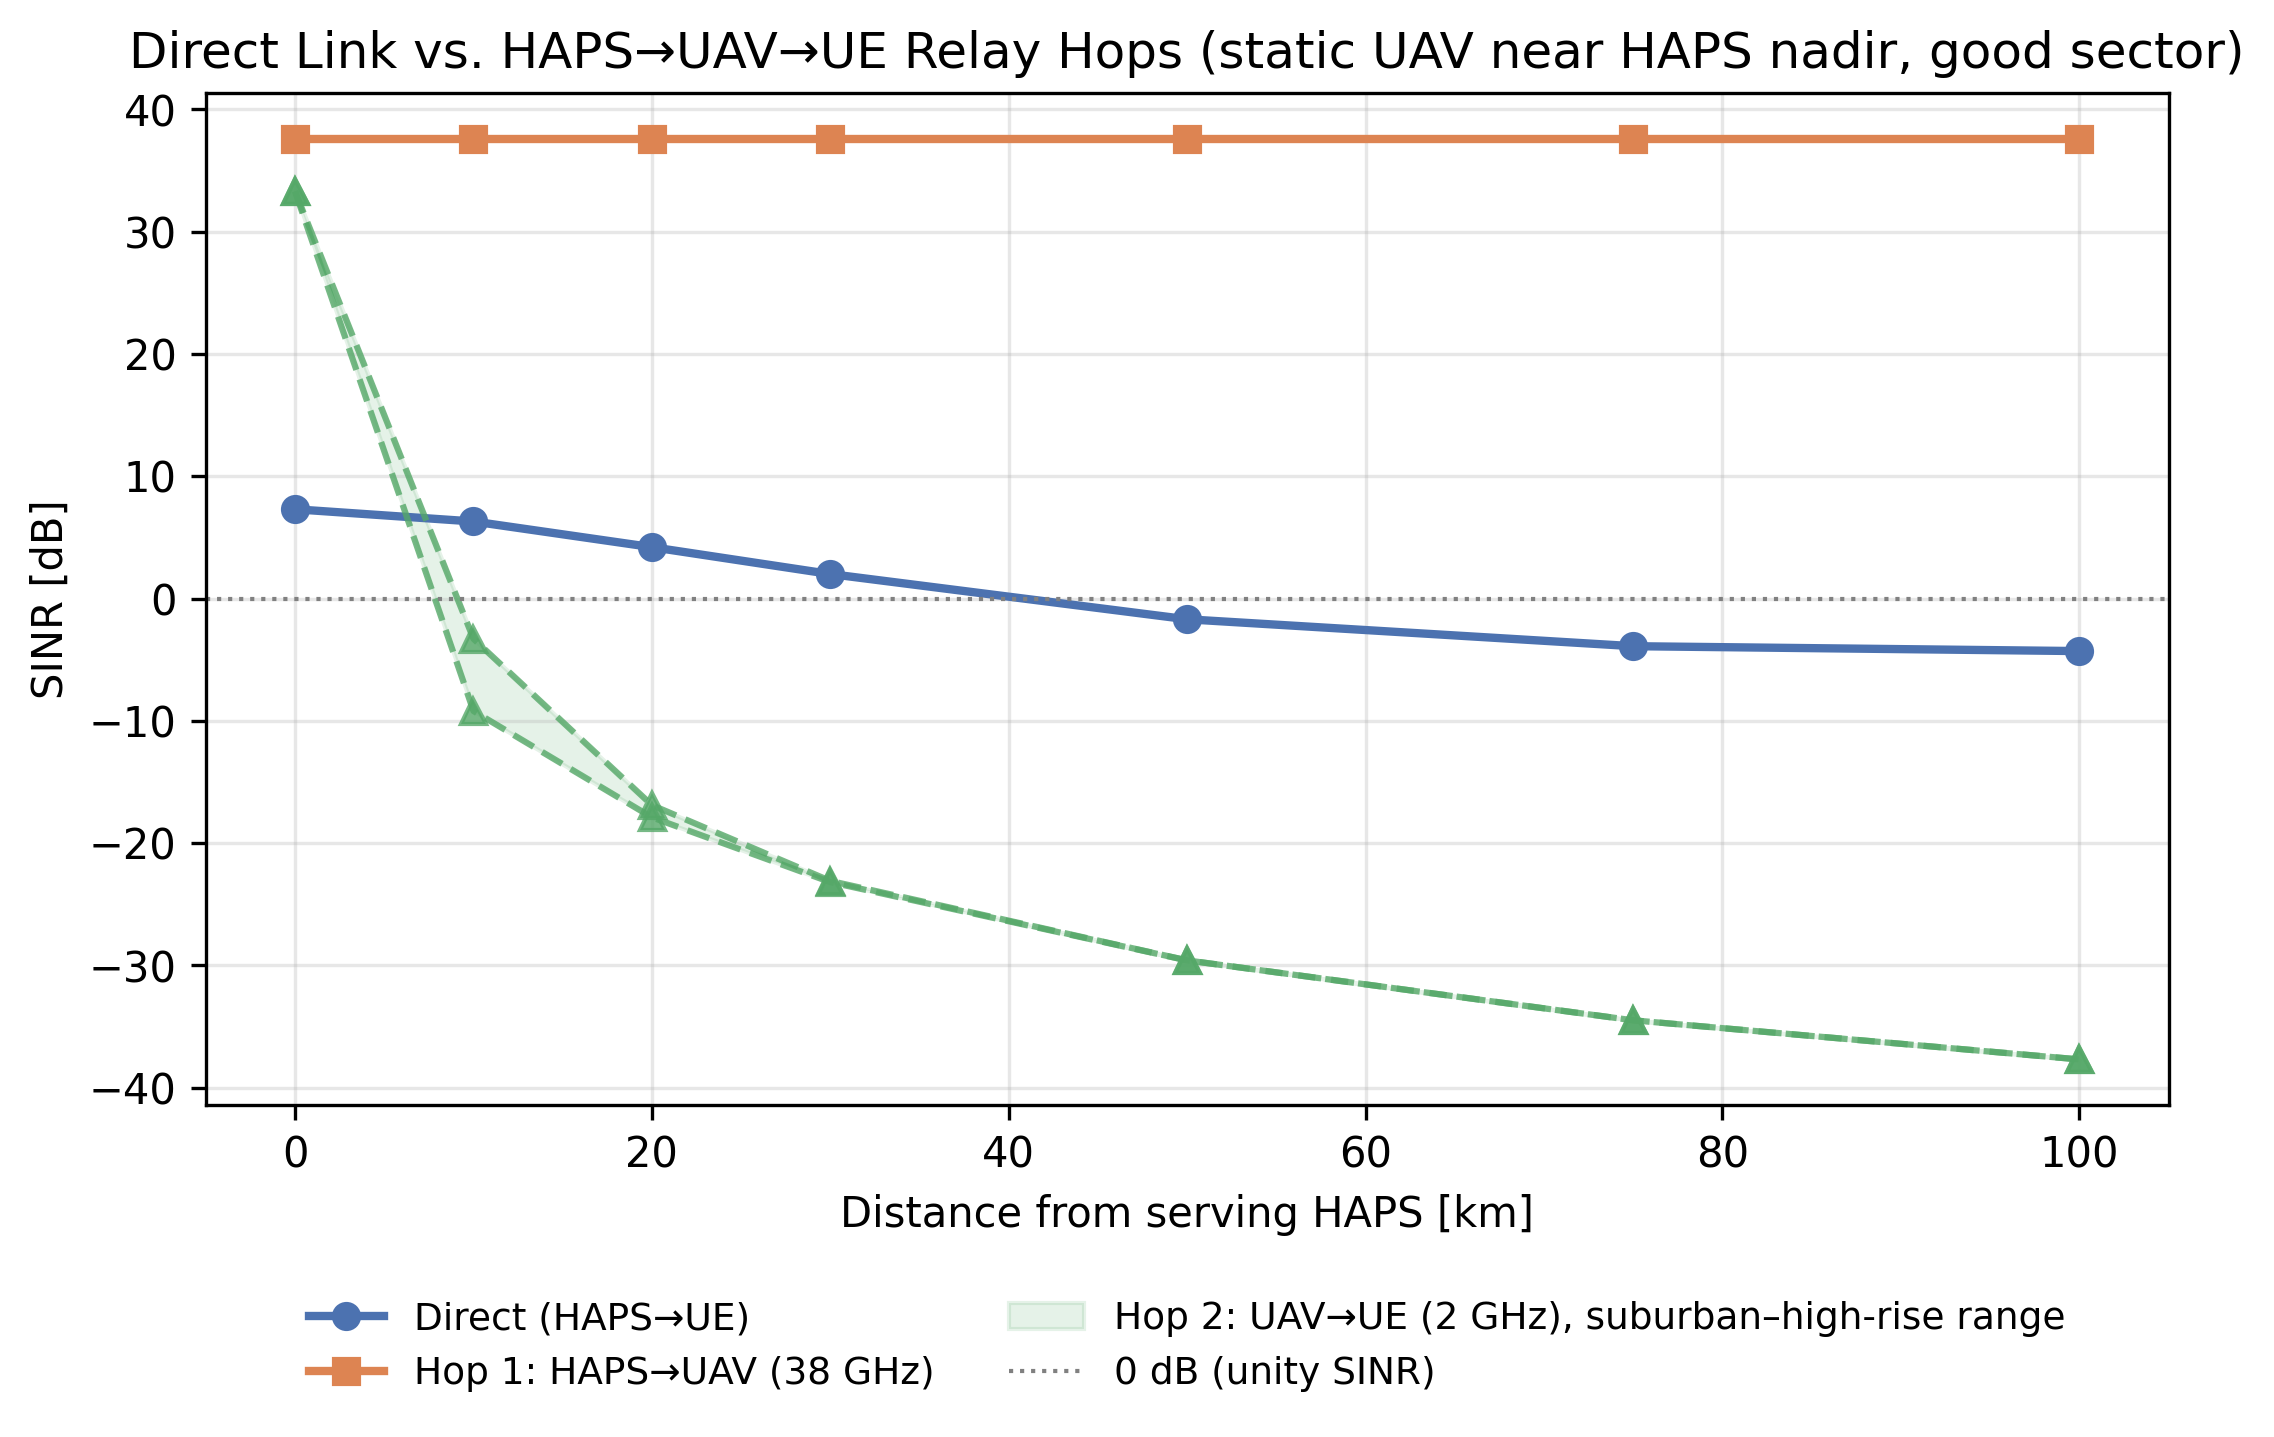
\includegraphics[width=\linewidth]{12_uav_relay_comparison.png}\\
\scriptsize\textbf{Relay hops vs.\ distance from serving HAPS} -- the
feeder hop (HAPS$\to$UAV) is flat at $10.2$\,bits/s/Hz by symmetry; the
access hop (UAV$\to$UE) collapses within a few km of the UAV's one
fixed position (next slide).
\end{column}
\begin{column}{0.33\textwidth}
\centering
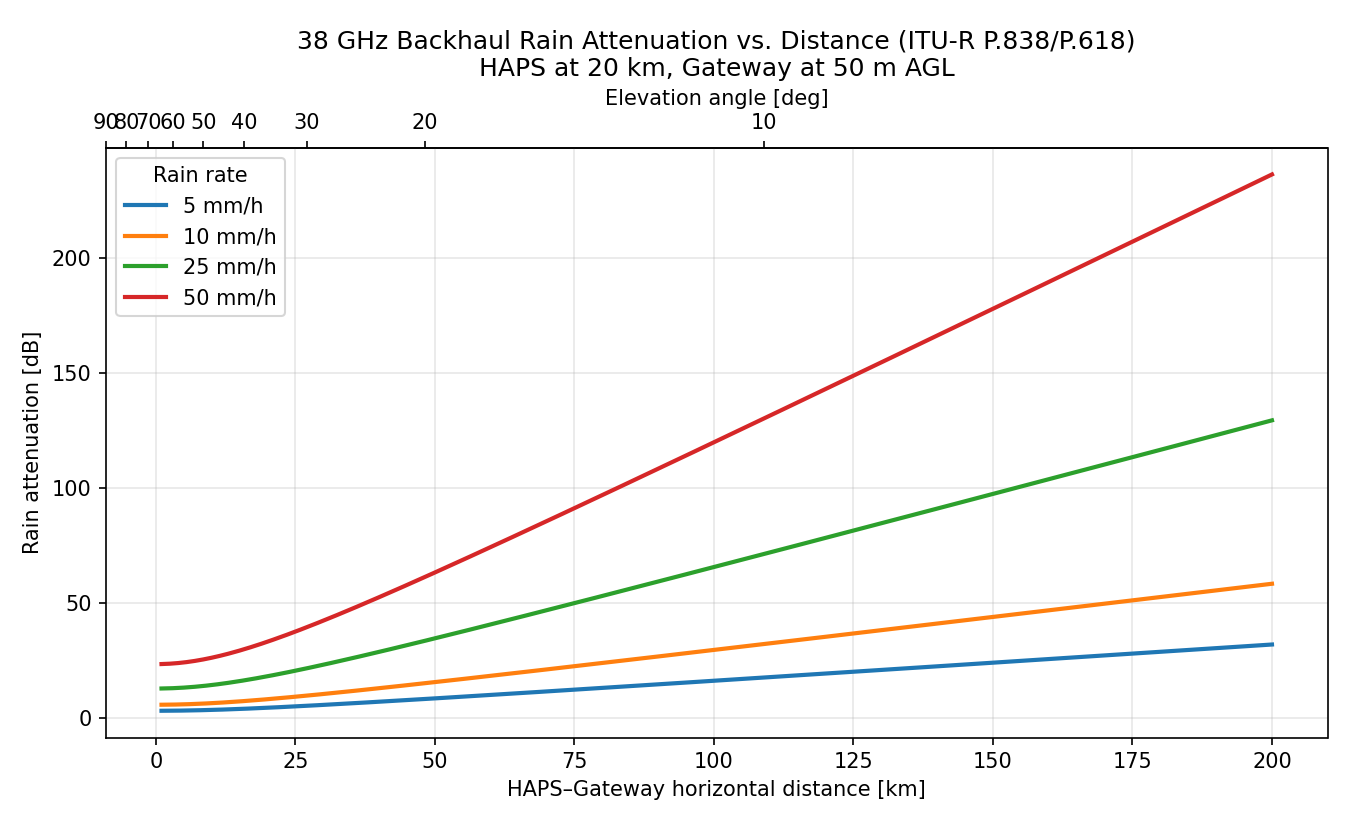
\includegraphics[width=\linewidth]{rain_attenuation_vs_distance.png}\\
\scriptsize\textbf{Rain attenuation vs.\ distance} (38\,GHz backhaul)
-- grows faster than linear past $\approx$100\,km as elevation drops
and the rain slant-path lengthens.
\end{column}
\end{columns}
\end{frame}

% ---------------------------------------------------------------
\begin{frame}{Why 38\,GHz: Frequency Selection}
\begin{columns}[T]
\begin{column}{0.48\textwidth}
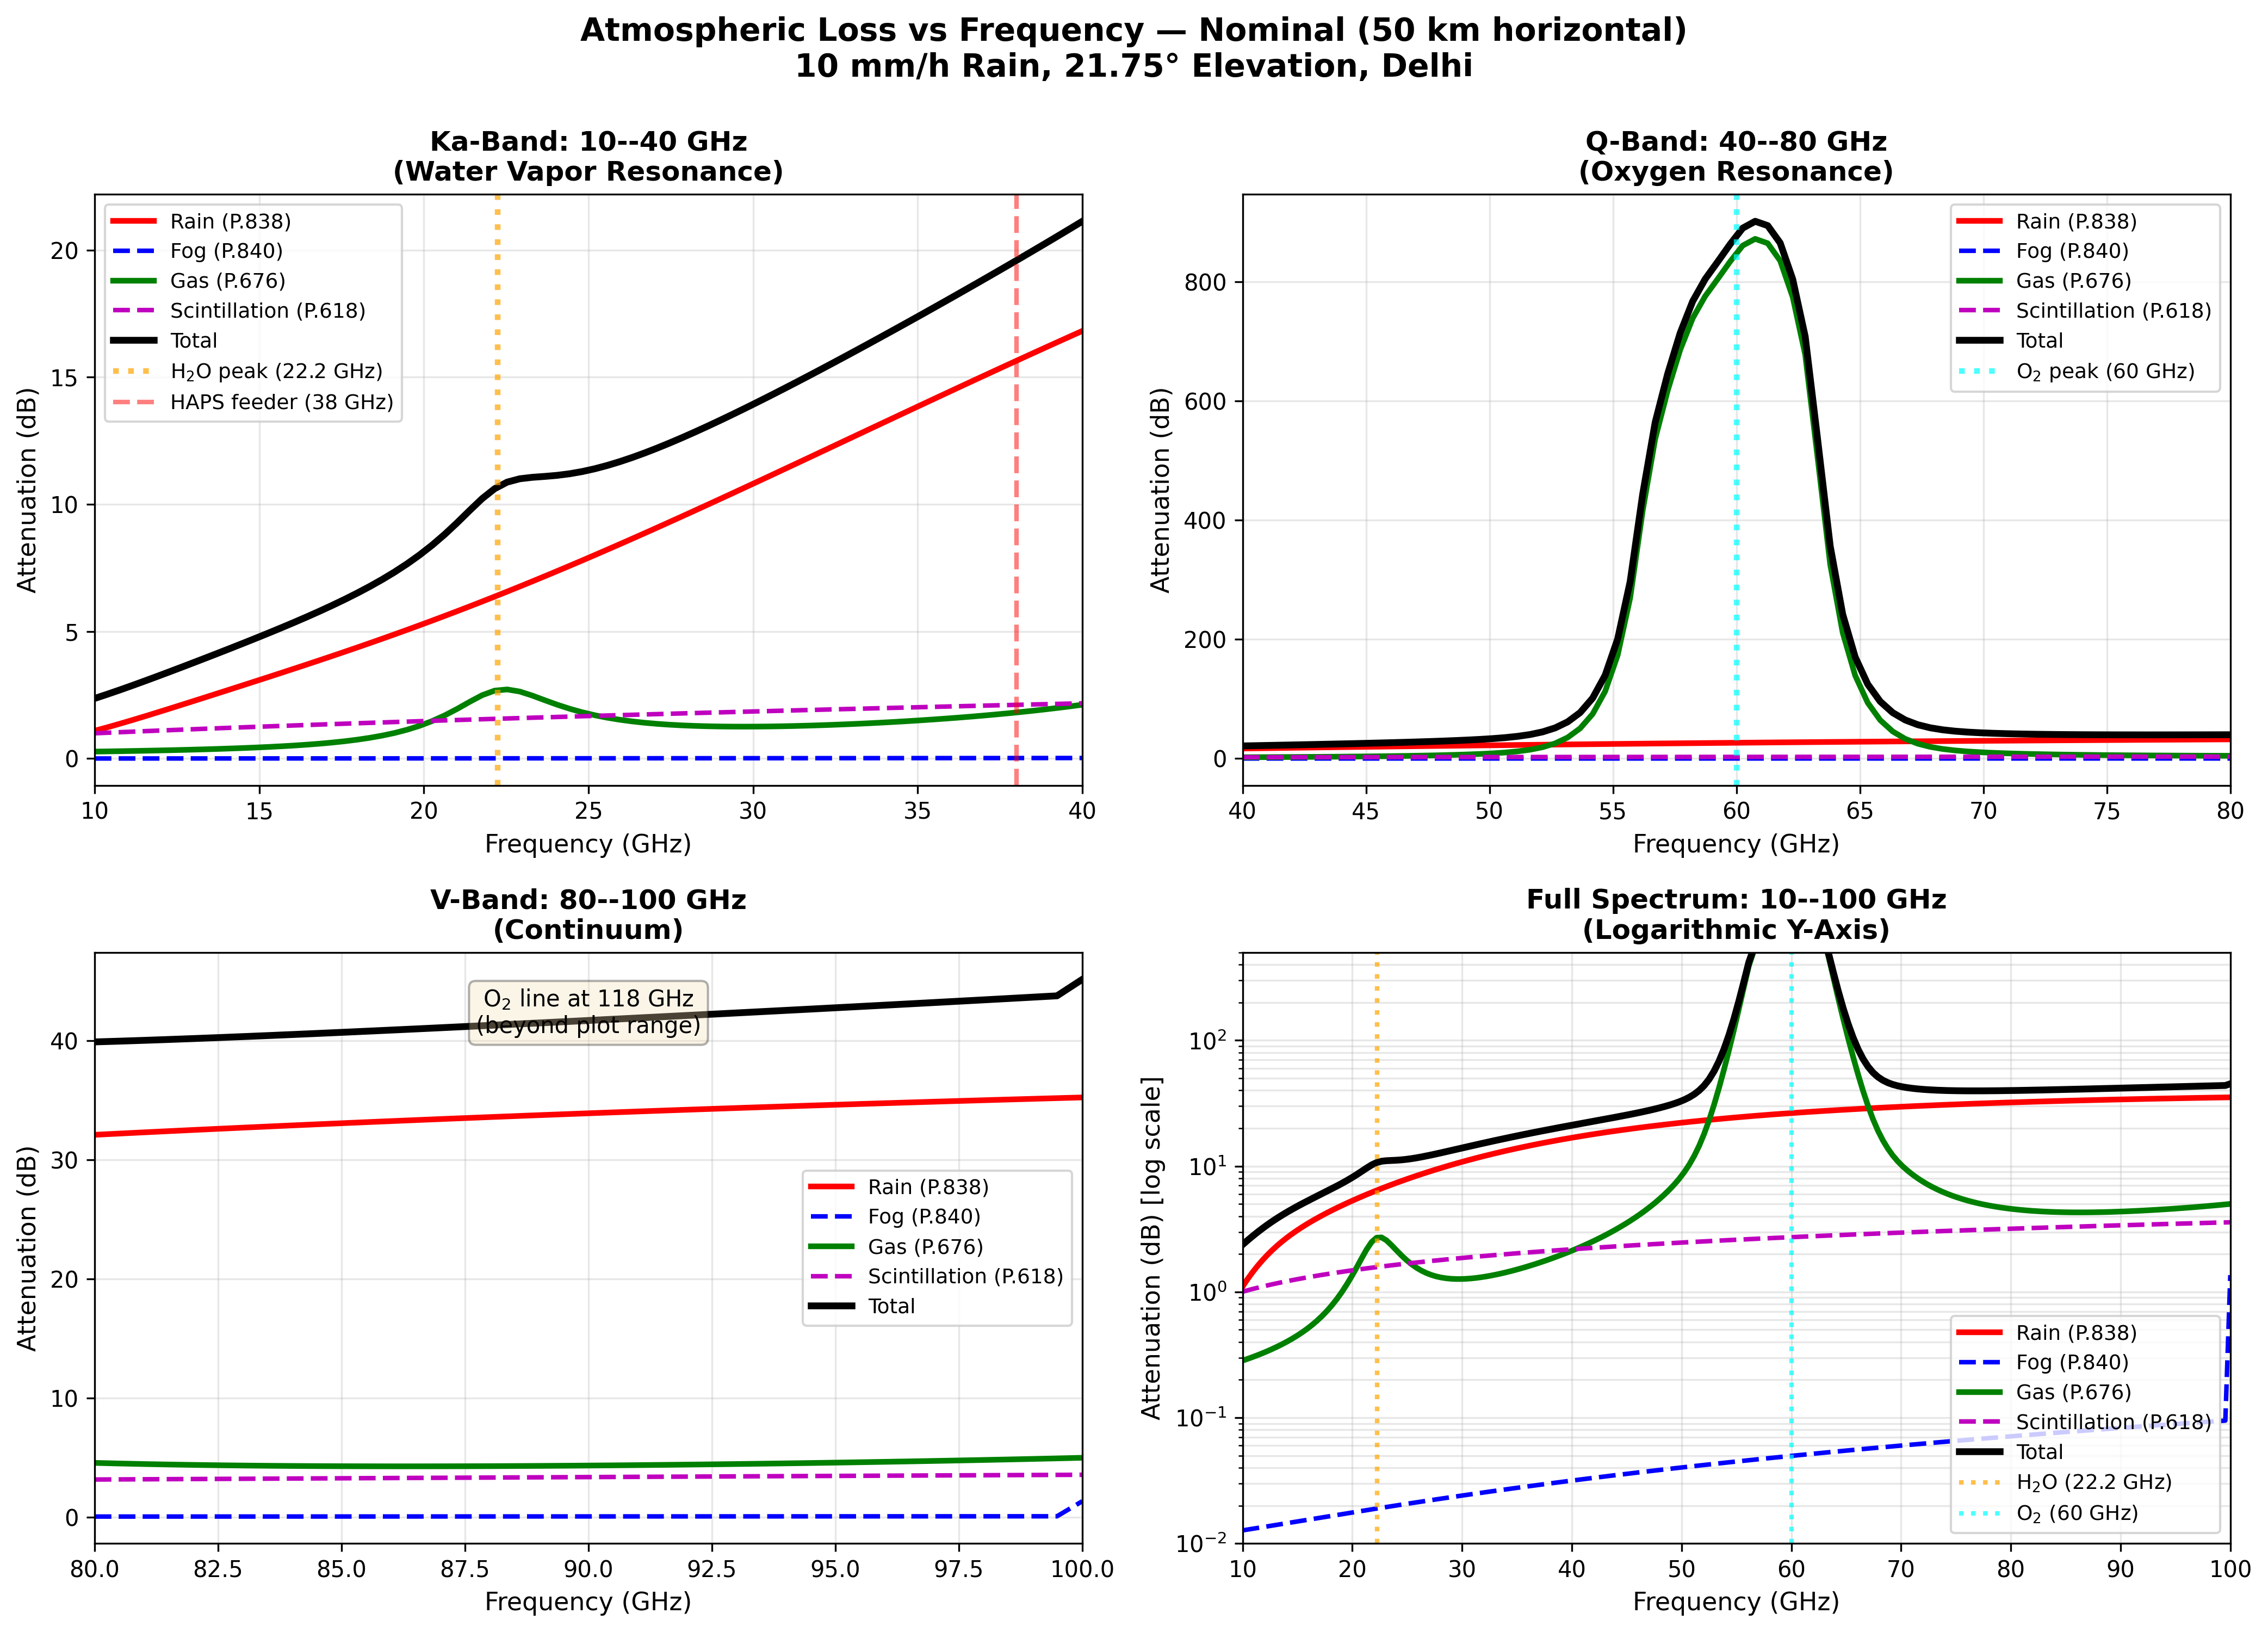
\includegraphics[width=\linewidth]{fig_atm_loss_nominal_frequency.png}
\end{column}
\begin{column}{0.52\textwidth}
\footnotesize
Atmospheric loss (rain, fog, gas) swept across the Ka/Q/V bands for
the Delhi gateway path, 10\,mm/h rain:
\begin{itemize}\setlength{\itemsep}{2pt}
  \item \textbf{Rain} (P.838/P.618) -- dominant term, grows roughly
        linearly with frequency; up to $\approx$19\,dB at 99.9\%
        availability ($R_{0.1}=15.7$\,mm/h).
  \item \textbf{Fog/cloud} (P.840) -- small except in dense fog;
        negligible below 10\,GHz.
  \item \textbf{Gas absorption} (P.676) -- two resonance peaks to
        avoid: H$_2$O at 22.2\,GHz, O$_2$ at 60\,GHz (there, total
        loss exceeds 800\,dB over 50\,km -- unusable).
\end{itemize}
\textbf{38\,GHz sits in the valley} between these peaks
($\approx$0.2--0.3\,dB/km clear-sky gas loss).
\vspace{2mm}

\scriptsize\textbf{The rain margin is not design, it's parameters:} with
literature-sourced hardware constants (43\,dBm Tx power, 13.8\,dBi
antenna gain), clear-sky backhaul SINR is $\approx$+38\,dB -- enough to
absorb the $\approx$19\,dB rain loss with $\approx$18.6\,dB left over.
This is a realistic margin (15--25\,dB is typical, ECC Report 156),
not something tuned by us.
\end{column}
\end{columns}
\end{frame}

% ---------------------------------------------------------------
\begin{frame}{Angular Interference Sectors and Scintillation Fading}
\begin{columns}[T]
\begin{column}{0.48\textwidth}
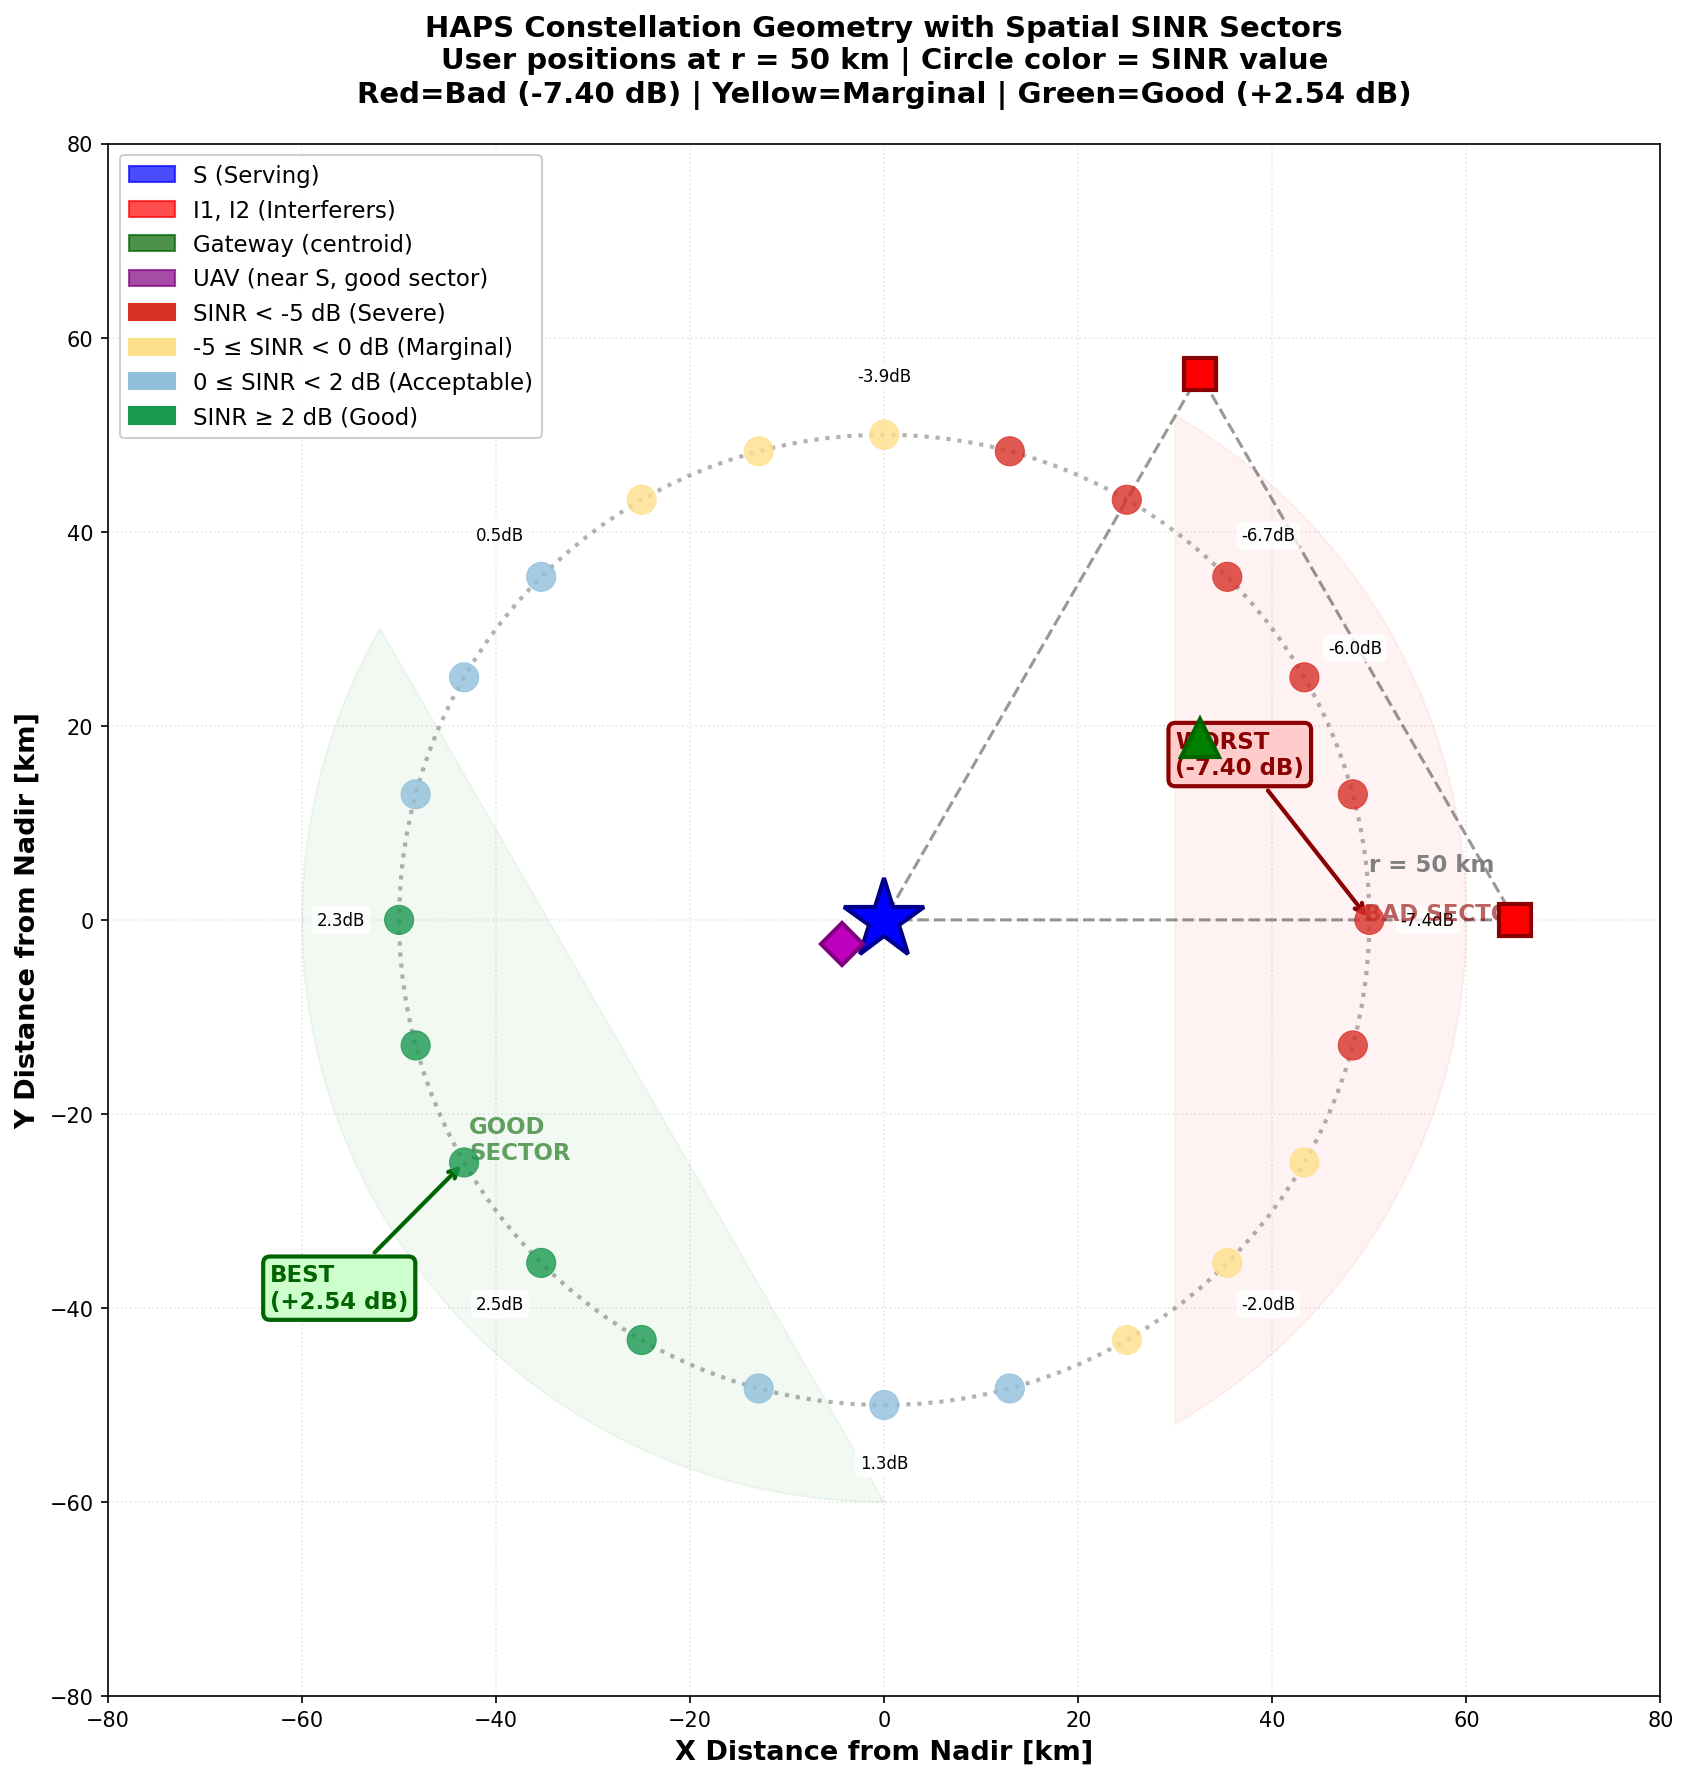
\includegraphics[width=\linewidth]{constellation_with_sectors.png}
\end{column}
\begin{column}{0.52\textwidth}
\footnotesize
\textbf{Angle-dependent SINR (sectors):} the 3-HAPS triangle creates a
good sector ($\approx$120\textdegree--290\textdegree, away from
interferers) and a bad sector ($\approx$330\textdegree--75\textdegree,
toward them) -- same radius, up to 9.94\,dB apart.

\vspace{2mm}
\textbf{Scintillation (ITU-R P.618):} rapid amplitude fluctuations
from tropospheric turbulence; grows with frequency, shrinks with
elevation. At 30\textdegree\ elevation, $p=0.01\%$: $\approx$0.49\,dB
at 38\,GHz vs.\ $\approx$0.09\,dB at 2.1\,GHz.

\vspace{2mm}
Favors positioning the UAV relay near nadir (higher elevation) when
feasible, especially for the HAPS--UAV feeder hop -- which also tends
to be away from the interferer-facing sector.

\vspace{2mm}
\scriptsize\textbf{Nuance:} each HAPS could simultaneously be a \emph{serving}
node (near-nadir, low-loss for its own users) and an \emph{interferer}
for the other two HAPS' users -- so this isn't a single clean
optimization across the constellation (future work, see Conclusion).
\end{column}
\end{columns}
\end{frame}

% ---------------------------------------------------------------
\begin{frame}{Why Learning is Needed: Spatial SINR Heterogeneity}
\begin{columns}[T]
\begin{column}{0.55\textwidth}
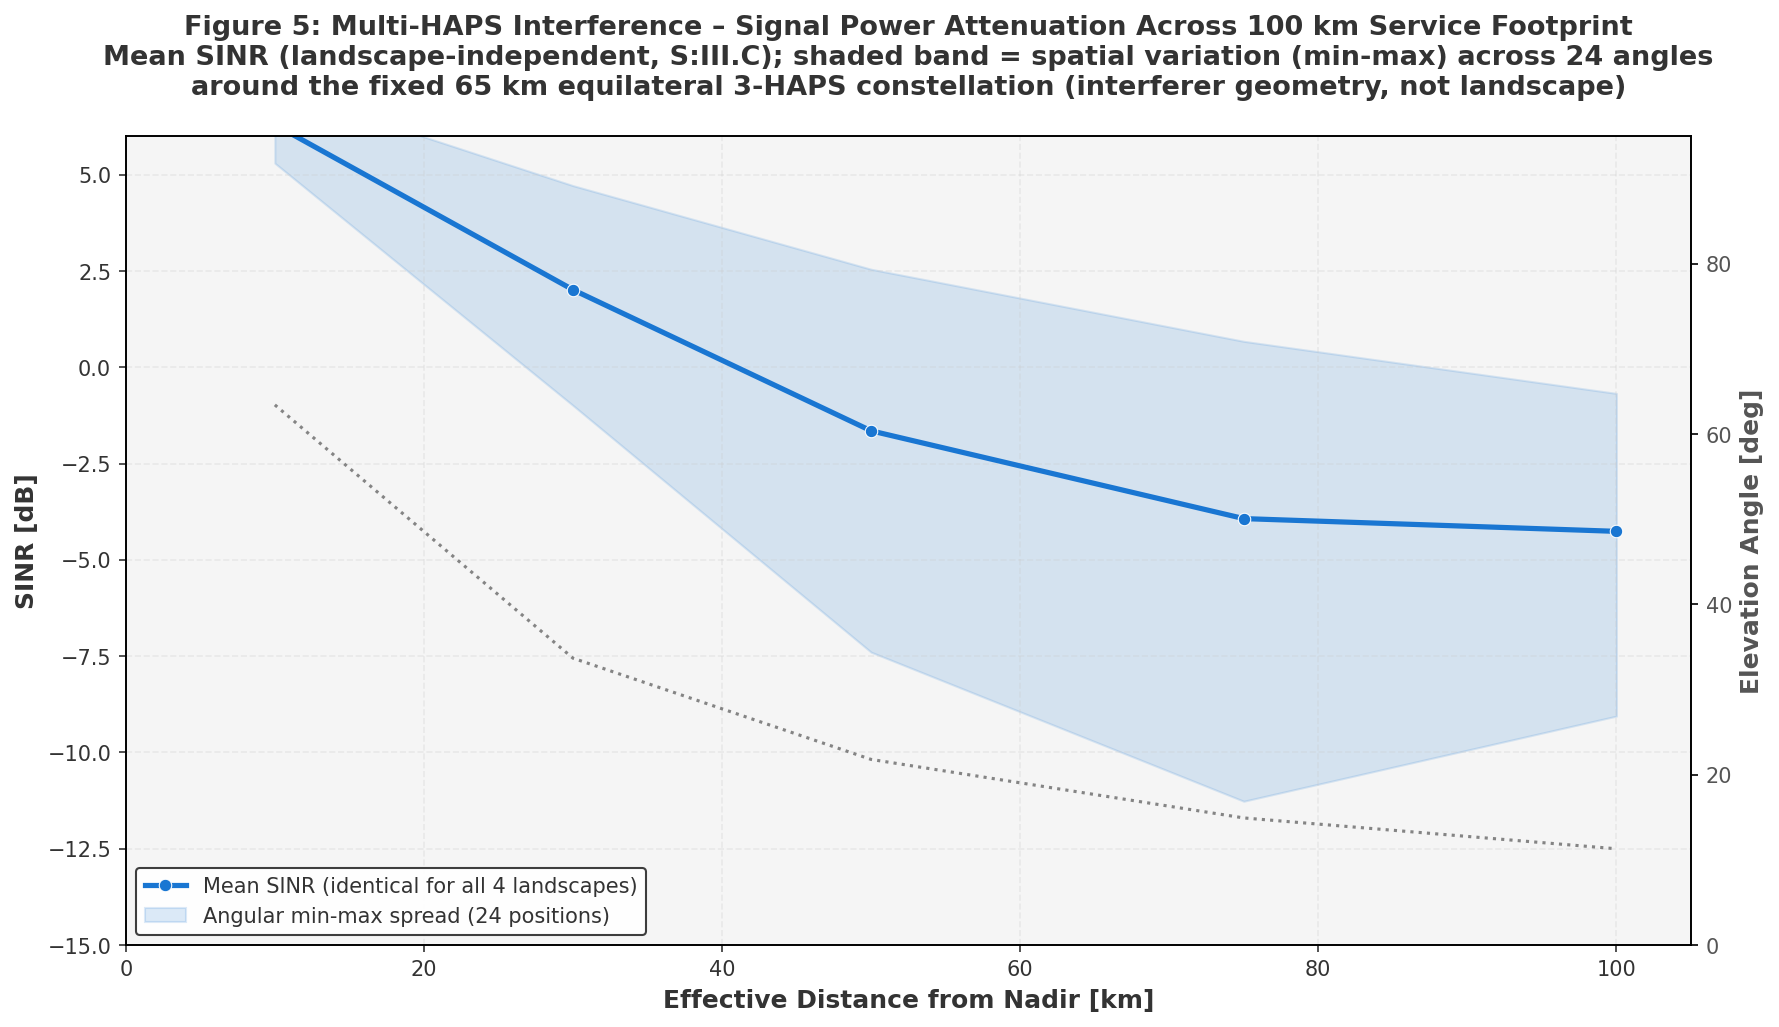
\includegraphics[width=\linewidth]{figure5_multi_haps_sinr_mean.png}
\end{column}
\begin{column}{0.45\textwidth}
\footnotesize
\begin{itemize}
  \item At a \textbf{fixed 50\,km radius}, SINR varies by
        \textbf{up to 9.94\,dB} depending on angular position relative to
        the two interfering HAPS.
  \item For comparison, simply \emph{doubling} the link distance only
        costs about 2--3\,dB -- so angular position affects SINR more
        than distance does.
  \item A simple ``always pick max-SINR'' rule cannot anticipate these
        angular patterns or adapt as weather and battery state change.
  \item \textbf{Conclusion:} a learned, real-time association policy is
        worth testing -- next slides show what it actually buys us.
\end{itemize}
\end{column}
\end{columns}
\end{frame}

% ---------------------------------------------------------------
\begin{frame}{The Relay UAV: One Static Platform, Not a Follower}
\footnotesize
\textbf{A key modeling correction:} the relay UAV is fixed 0.1\,km from
the serving HAPS's own nadir (elevation $\approx$89.71$^\circ$; the
Gateway occupies the centroid instead, circumradius $\approx$37.5\,km,
elevation $\approx$27.995$^\circ$) -- it does \emph{not} hover beside
whichever user it currently serves. One UAV cannot be everywhere at once.
\vspace{2mm}
\begin{itemize}\setlength{\itemsep}{3pt}
  \item \textbf{Feeder hop (HAPS$\to$UAV):} constant geometry $\Rightarrow$
        constant capacity, $12.48$\,bits/s/Hz, for every HAPS by the
        constellation's symmetry.
  \item \textbf{Access hop (UAV$\to$UE):} depends on the user's \emph{real}
        distance from that one fixed point -- capacity falls from
        $11.1$\,bits/s/Hz at the UAV's own location to $0.96$\,bits/s/Hz
        at 5\,km and $0.17$\,bits/s/Hz at 10\,km (urban terrain; unchanged
        from the previous centroid-UAV geometry). Usable radius (capacity
        $>0.5$\,bits/s/Hz): $\approx$6.5\,km (urban) to 10.3\,km (suburban).
  \item Raw capacity: relay \emph{exceeds} the direct link's within
        $\approx$1--6\,km of the serving HAPS's own nadir, falling to
        $0.50$\,bits/s/Hz (direct: $\approx$2.5--2.6) at $R_\mathrm{eff}$.
  \item Contention: one HAPS's direct-link population ($100^2/3$, full
        footprint) outnumbers one UAV's relay population
        ($R_\mathrm{eff}^2$, its own disk) by $\approx$79:1 urban,
        31:1 suburban -- pure geometry, population density cancels.
  \item Per-user share: relay beats direct \emph{everywhere} inside
        $R_\mathrm{eff}$ once this is priced in -- 15x at the urban
        disk's own edge, 6x suburban; more near the UAV. Beyond
        $R_\mathrm{eff}$, how far this extends is open.
  \item Full, gap-free coverage of a 100\,km service radius would still
        need $\sim$200--270 such UAVs (a covering-number estimate),
        placed away from each HAPS's own nadir -- a
        fleet-assignment problem, not a scaled-up version of today's
        single-UAV model (future work).
\end{itemize}
\end{frame}

% ---------------------------------------------------------------
\begin{frame}{LSTM Rain-Attenuation Forecaster}
\begin{columns}[T]
\begin{column}{0.48\textwidth}
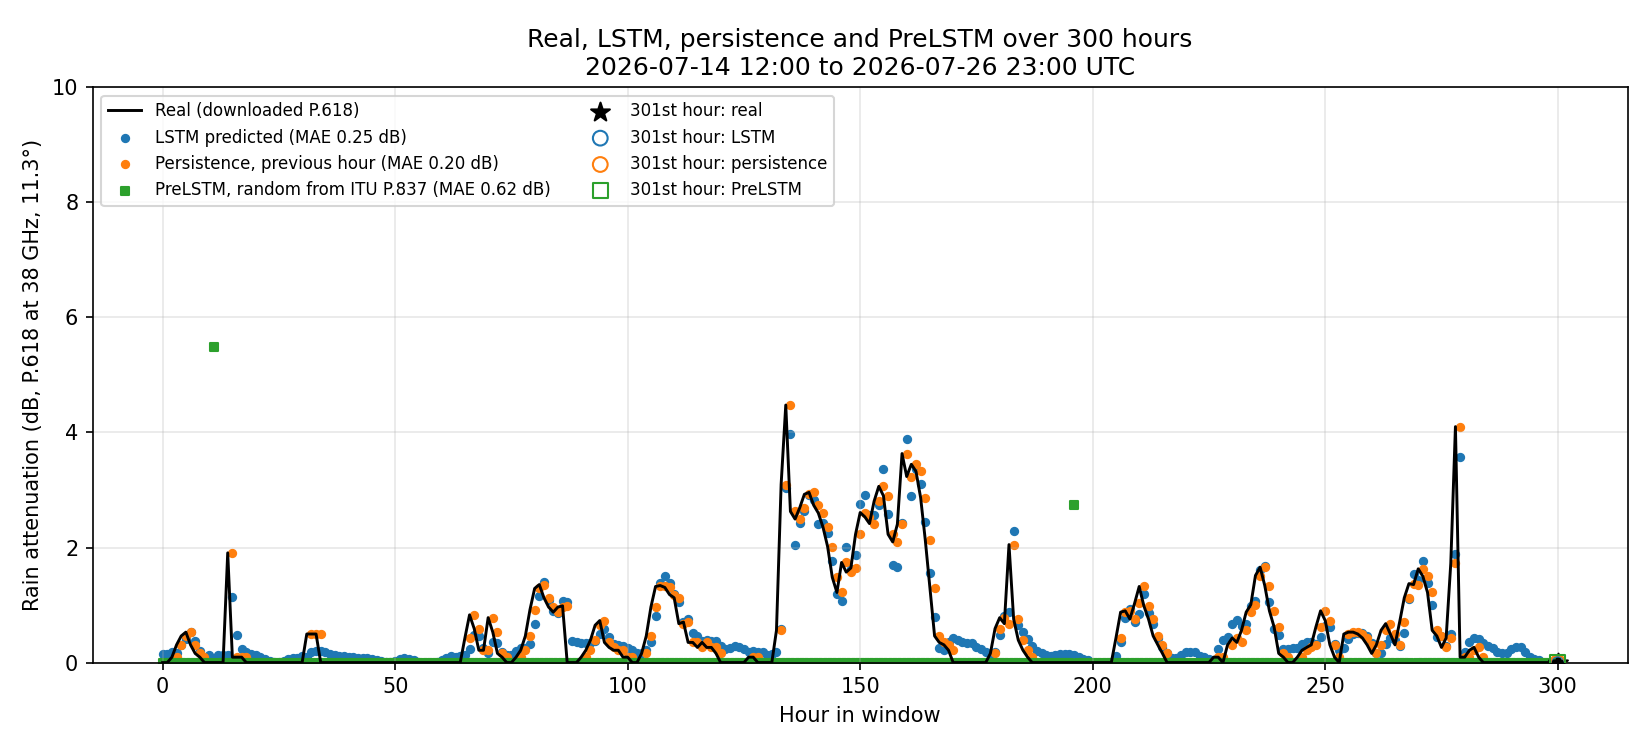
\includegraphics[width=\linewidth]{lstm_forecast_2026.png}
\vspace{2mm}
\footnotesize
\begin{itemize}\setlength{\itemsep}{2pt}
  \item DQN must decide at hour $t$ \emph{before} that hour's rain is
        observed $\Rightarrow$ needs a forecast.
  \item Evaluated \textbf{out-of-sample} (2026 forecasts from a model
        trained only on 2023--2025 data).
  \item Properly \textbf{early-stopped}: validation (2025) RMSE is best
        at epoch 4, not 30 -- training longer overfits (next slide).
\end{itemize}
\end{column}
\begin{column}{0.52\textwidth}
\footnotesize
\begin{itemize}\setlength{\itemsep}{2pt}
  \item LSTM predicts feeder (38\,GHz) rain attenuation up to
        \textbf{six hours ahead} from NASA POWER / METAR / ERA5 weather
        history for Delhi.
  \item At this validated stopping point, the LSTM beats persistence
        on RMSE at every horizon from $+2$\,h onward (Table, next slide);
        persistence only wins at $+1$\,h.
  \item A validated, per-horizon-weighted ensemble of LSTM + persistence
        (weight chosen on 2025, applied once to 2026) adds a small
        further gain at the shortest horizon.
  \item \textbf{But:} a more accurate forecast $\neq$ a forecast the DQN
        can use -- see the ablation result ahead.
\end{itemize}
\end{column}
\end{columns}
\end{frame}

% ---------------------------------------------------------------
\begin{frame}{LSTM vs.\ Persistence, 2026 Test Set}
\footnotesize
\begin{table}
\centering
{\scriptsize
\begin{tabularx}{\linewidth}{|>{\centering\arraybackslash}X|>{\centering\arraybackslash}X|>{\centering\arraybackslash}X|>{\centering\arraybackslash}X|>{\centering\arraybackslash}X|}
\hline
\textbf{Horizon} & \textbf{LSTM MAE} & \textbf{Persist.\ MAE} & \textbf{LSTM RMSE} & \textbf{Persist.\ RMSE} \\
\hline
$+1$\,h & $0.15$ & $\mathbf{0.12}$ & $0.54$ & $\mathbf{0.53}$ \\
\hline
$+2$\,h & $0.21$ & $\mathbf{0.20}$ & $\mathbf{0.70}$ & $0.75$ \\
\hline
$+3$\,h & $\mathbf{0.24}$ & $0.26$ & $\mathbf{0.80}$ & $0.90$ \\
\hline
$+4$\,h & $\mathbf{0.27}$ & $0.30$ & $\mathbf{0.86}$ & $1.02$ \\
\hline
$+5$\,h & $\mathbf{0.28}$ & $0.34$ & $\mathbf{0.90}$ & $1.11$ \\
\hline
$+6$\,h & $\mathbf{0.29}$ & $0.36$ & $\mathbf{0.92}$ & $1.17$ \\
\hline
\end{tabularx}}
\end{table}
\begin{itemize}
  \item 6556 forecast hours, 2026, no 2026 data in training.
  \item Persistence only wins at the shortest horizon ($+1$\,h) -- little
        changes in an hour, so ``tomorrow looks like now'' is hard to beat.
  \item The LSTM's advantage grows with horizon as its learned dynamics
        start to matter more than the last observed value.
\end{itemize}
\end{frame}

% ---------------------------------------------------------------
\begin{frame}{DQN Association Agent: Problem Formulation}
\footnotesize
\textbf{Per-user MDP} -- each user independently chooses a platform; network
reward is computed after all assignments.
\vspace{2mm}

\begin{columns}[T]
\begin{column}{0.48\textwidth}
\begin{itemize}\setlength{\itemsep}{3pt}
  \item \textbf{State:} SINR to each platform, distance, battery SoC,
        rainfall, visibility, time-of-day, six LSTM rain forecasts.
  \item \textbf{Action:} $a_k \in \{0,\dots,5\}$ -- direct link to
        HAPS1--3, or relay through the one UAV served by HAPS1--3.
\end{itemize}
\end{column}
\begin{column}{0.52\textwidth}
\begin{itemize}\setlength{\itemsep}{3pt}
  \item \textbf{Reward:} throughput (rain-derated) + fairness (Jain
        index) $-$ energy cost $-$ outage/degraded-service penalties
        $-$ low-battery penalty.
\end{itemize}
\vspace{2mm}
\begin{itemize}\setlength{\itemsep}{3pt}
  \item Custom Deep Q-Network implemented directly in PyTorch
        (\texttt{torch}/\texttt{torch.nn}).
  \item Trained on \textbf{2400} rolling 24-hour episodes (400 real
        2024 episodes, cycled six times -- 400 alone left reward still
        improving noisily); evaluated on 50 held-out 2025 days,
        \textbf{ten} experiments (random seeds).
\end{itemize}
\end{column}
\end{columns}
\end{frame}

% ---------------------------------------------------------------
\begin{frame}{Results: Policy Comparison}
\footnotesize
\begin{table}
\centering
\begin{tabularx}{\linewidth}{|>{\raggedright\arraybackslash}X|>{\centering\arraybackslash}X|>{\centering\arraybackslash}X|>{\centering\arraybackslash}X|}
\hline
\textbf{Policy} & \textbf{Reward/step} & \textbf{Jain} & \textbf{Outage/50} \\
\hline
Random (six actions) & $-92.2\,(1.4)$ & $0.255\,(0.011)$ & $41.6\,(0.3)$ \\
\hline
Max-SINR (direct only) & $-14.5\,(1.7)$ & $\mathbf{0.558}\,(0.013)$ & $\mathbf{0.8}\,(0.2)$ \\
\hline
Max-throughput (six actions) & $\mathbf{-14.6}\,(1.7)$ & $0.241\,(0.039)$ & $\mathbf{0.8}\,(0.2)$ \\
\hline
LSTM + DQN & $-15.1\,(1.7)$ & $0.351\,(0.112)$ & $1.2\,(0.2)$ \\
\hline
\end{tabularx}
\end{table}
\begin{itemize}
  \item Mean $\pm$ std.\ dev.\ over ten experiments, 50 held-out 2025 days.
  \item The DQN is behind both rule-based baselines on reward and
        outage, and behind max-SINR on fairness -- but \textbf{fairer
        than max-throughput} (Jain $0.351$ vs.\ $0.241$, 8/10 seeds),
        once per-HAPS and per-UAV contention is modelled.
  \item Max-SINR and Max-throughput are both \textbf{oracle-style upper
        bounds}: perfect, instantaneous SINR/capacity knowledge, no
        learning, no real deployability constraint. The DQN was never
        expected to beat them -- the honest question is what it gets
        right that they can't (two slides ahead).
\end{itemize}
\end{frame}

% ---------------------------------------------------------------
\begin{frame}{Results: Stability Across Experiments}
\begin{columns}[T]
\begin{column}{0.48\textwidth}
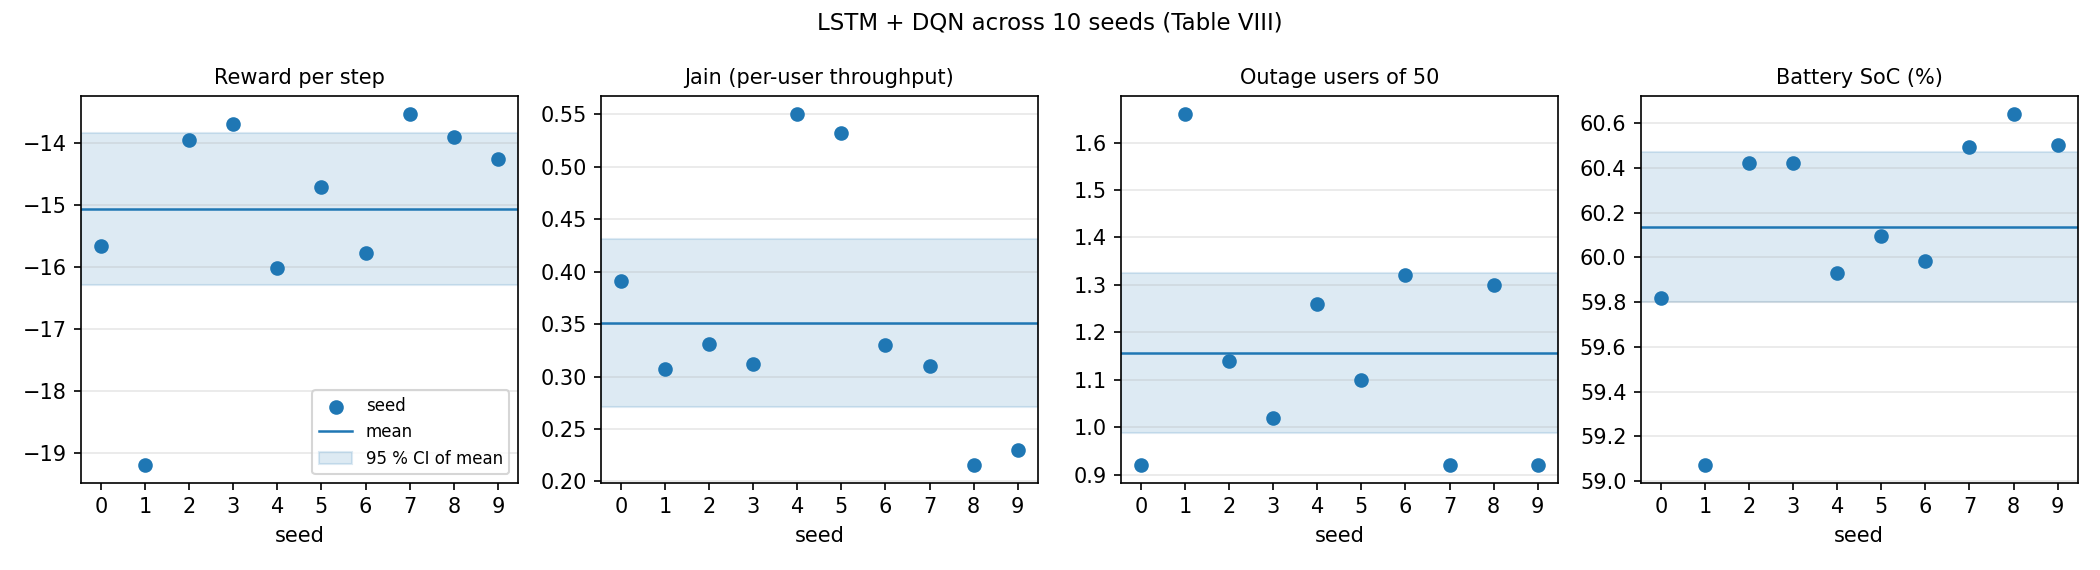
\includegraphics[width=\linewidth]{seed_stats.png}
\vspace{2mm}
\scriptsize
\textbf{LSTM + DQN, ten independent seeds} (dot = one training run;
line = mean; band = 95\% CI \emph{of the mean}):
\begin{itemize}\setlength{\itemsep}{0pt}
  \item Reward/step: $-15.07 \pm 1.71$ \\ (95\% CI $[-16.30, -13.85]$)
  \item Jain fairness: $0.351 \pm 0.112$
  \item Outage: $1.16 \pm 0.24$ of 50 users
  \item Battery SoC: $60.14 \pm 0.47\,\%$
\end{itemize}
\end{column}
\begin{column}{0.52\textwidth}
\scriptsize
\textbf{CI vs.\ spread:} the shaded band is \emph{not} ``most runs land
here'' -- it narrows with more seeds even if run-to-run variability
stays the same. It shows how precisely the \emph{true mean} is known
from these ten runs.

\vspace{2mm}
\textbf{Takeaway:} the tight spread across all ten seeds shows the
policy is \textbf{reliably learned to this level}, not a lucky or
unlucky single run -- consistency, not the reward level itself, is
what this figure demonstrates.
\end{column}
\end{columns}
\end{frame}

% ---------------------------------------------------------------
\begin{frame}{Results: Statistical Significance}
\begin{columns}[T]
\begin{column}{0.42\textwidth}
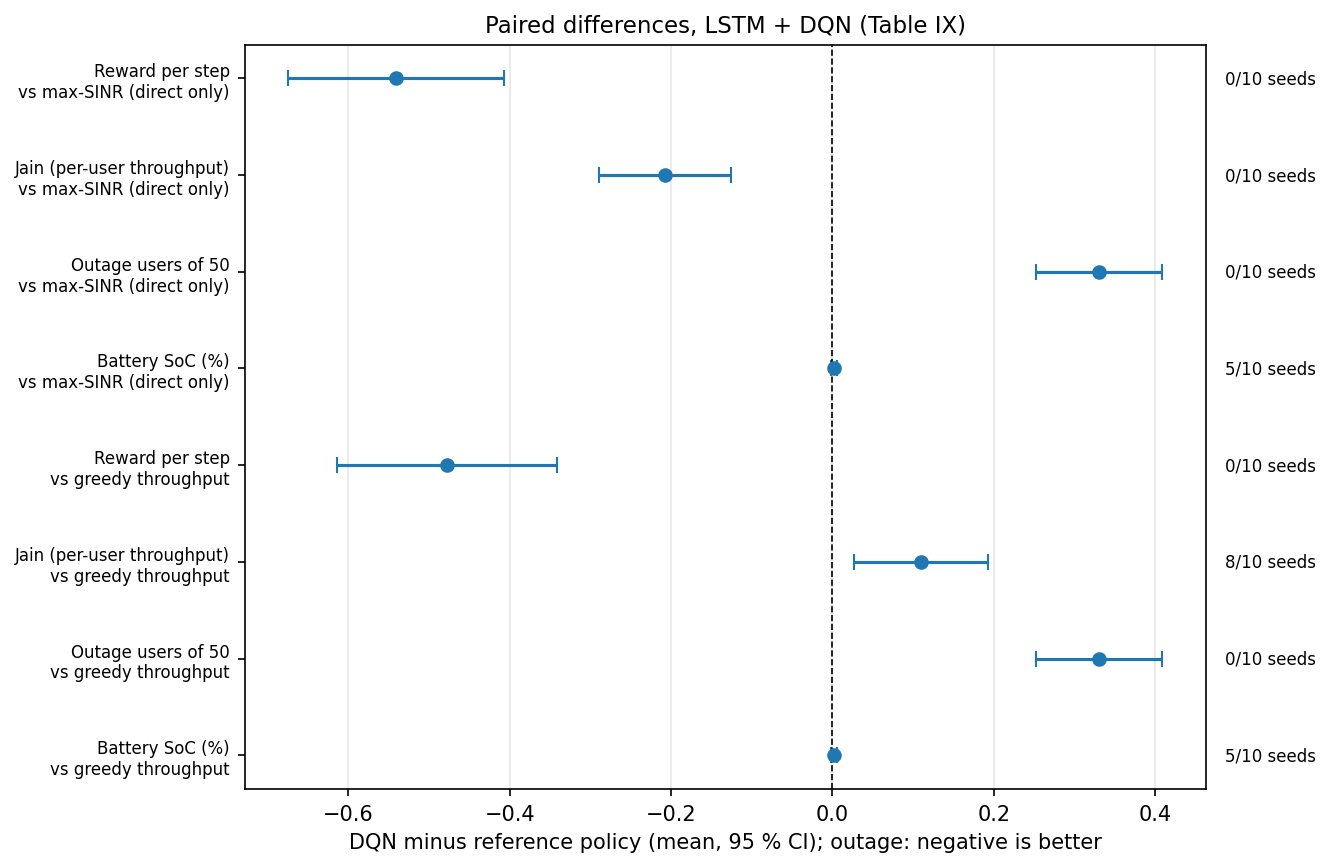
\includegraphics[width=\linewidth]{paired_forest.png}
\end{column}
\begin{column}{0.58\textwidth}
\scriptsize
Paired differences, LSTM+DQN minus baseline (per experiment, 50 days
each, ten seeds). Whiskers crossing 0 = not significant.

\vspace{1mm}
\textbf{vs.\ Max-SINR:}
\begin{itemize}\setlength{\itemsep}{0pt}
  \item Reward: $-0.54$ ($p<0.0001$) -- DQN worse, 0/10
  \item Jain: $-0.207$ ($p=0.0003$) -- DQN worse, 0/10
  \item Outage: $+0.33$ ($p<0.0001$) -- DQN worse, 0/10
  \item Battery SoC: $\approx0$ ($p=0.33$) -- tie
\end{itemize}

\vspace{1mm}
\textbf{vs.\ Max-throughput:}
\begin{itemize}\setlength{\itemsep}{0pt}
  \item Reward: $-0.48$ ($p<0.0001$) -- DQN worse, 0/10
  \item Jain: $\mathbf{+0.110}$ ($p=0.0153$) -- \textbf{DQN fairer}, 8/10
  \item Outage: $+0.33$ ($p<0.0001$) -- DQN worse, 0/10
  \item Battery SoC: $\approx0$ ($p=0.33$) -- tie
\end{itemize}

\vspace{1mm}
\textbf{Takeaway:} the DQN loses to both oracle-style baselines on
reward and outage on nearly every seed, and to max-SINR on fairness --
but is fairer than max-throughput on 8/10 seeds, once per-HAPS and
per-UAV contention is modelled.
\end{column}
\end{columns}
\end{frame}

% ---------------------------------------------------------------
\begin{frame}{What the DQN Gets Right That the Baselines Can't}
\footnotesize
\begin{itemize}\setlength{\itemsep}{4pt}
  \item Max-SINR needs only a real-time SINR reading -- already a
        deployable rule, but cannot use relay at all. Max-throughput
        needs perfect, instantaneous, non-causal knowledge of every
        option's capacity including relay -- not deployable, and its
        own fairness collapses (Jain $0.241$) once contention is
        modelled, since it loads every crowded user onto the same
        best-looking option with no notion of who else is using it.
  \item \textbf{The DQN is the only policy that retains and actually
        uses the relay path} -- which, once per-HAPS vs.\ per-UAV
        contention is modelled, beats direct everywhere inside its own
        disk (previous slides), not just for a narrow subset of users.
  \item So the DQN's value is \textbf{structural} (targeted relay
        fallback for near-outage users), not a reward-table win against
        oracle-style baselines that were never realistic competitors.
\end{itemize}
\end{frame}

% ---------------------------------------------------------------
\begin{frame}{Does the Rain Forecast Help the DQN Itself?}
\footnotesize
A forecast ablation (\texttt{lstm} vs.\ \texttt{none} -- forecast
features zeroed -- vs.\ \texttt{oracle} -- true future attenuation),
same ten-seed protocol:
\vspace{2mm}
\begin{itemize}\setlength{\itemsep}{4pt}
  \item \textbf{Result:} \texttt{lstm}, \texttt{none}, and
        \texttt{oracle} are statistically indistinguishable on reward,
        fairness, and outage (all $p>0.1$) -- even against the oracle
        ceiling, and it stays null after two further tests.
  \item \textbf{Gave the UAV feeder its own rain fade} (previously
        unmodelled; its near-zenith path fades \emph{more} than the
        backhaul's at most rain rates). Still null.
  \item \textbf{Added a per-user switching-cost penalty}, testing
        whether reacting late is the missing friction. Still null --
        with one UAV, there's no penalty-free alternative to
        pre-emptively move traffic to.
  \item \textbf{Why:} this MDP lets every user react to the current
        hour's rain for free -- raw rain rate is already a state
        feature regardless of the forecast. A forecast only pays off
        when reacting late costs something real.
  \item \textbf{Where it would matter:} a fleet, where a fade over one
        HAPS squeezes every UAV feeding off it at once -- a
        synchronized surge only foresight can stagger.
\end{itemize}
\end{frame}

% ---------------------------------------------------------------
\begin{frame}{Conclusion and Future Work}
\scriptsize
\textbf{Channel model.} Spatial SINR heterogeneity (up to 9.94\,dB at
fixed 50\,km) dominates service-link quality; backhaul remains
noise-limited. \quad
\textbf{Relay path.} A single static UAV fixed 0.1\,km from the serving
HAPS's own nadir has a collapsing access hop -- but once contention is
modelled (one HAPS's direct-link crowd is $\approx$79x a UAV's relay
crowd, by geometry alone), relay beats direct \emph{everywhere} inside
its own $\approx$6.5--10.3\,km disk. One UAV still only covers that
one disk; full coverage would need $\sim$200--270 such UAVs placed
away from each HAPS's own nadir. \quad
\textbf{Learned association.} The LSTM-fed DQN is behind Max-SINR and
Max-throughput on reward and outage, behind Max-SINR on fairness, but
fairer than Max-throughput once contention is modelled -- and is the
only policy that targets relay use at users who actually need it. The
rain forecast adds no measurable reward benefit even after two further
tests (feeder's own rain fade, switching-cost penalty); a fleet, where
a fade forces a synchronized multi-UAV surge, is where it should start
to matter.

\vspace{2mm}
\textbf{Future work:}
\begin{itemize}\setlength{\itemsep}{0pt}
  \item \textbf{Model multiple UAVs:} HAPS-to-UAV assignment as its own
        fleet-scale MDP, decoupled from per-user access; relay-vs-direct
        as an explicit policy layer; relative motion of UAVs and HAPS;
        fleet placement that avoids blind corners.
  \item \textbf{LSTM improvements:} alternative architectures (ConvLSTM,
        GRU, spatio-temporal GNNs for irregular future sites); the
        validated ensembling gain already found; forecasting a
        different impairment if time-series data for it existed (fog,
        scintillation, gas) -- rain was the only one we had multi-year
        data for.
  \item \textbf{Dynamic topology and geometry:} changing HAPS roles
        (serving vs.\ interferer); joint UAV/HAPS positioning across
        both roles at once; beamforming between HAPS and Gateway.
\end{itemize}

\vspace{2mm}
\centering \large Thank you -- Questions?
\end{frame}

\end{document}
